%%%%%%%%%%%%%%%%%%%%%%%%%%%%%%%%%%%%%%%%%%%%%%%%%%%%
%%%             Metadata                         %%%
%%%%%%%%%%%%%%%%%%%%%%%%%%%%%%%%%%%%%%%%%%%%%%%%%%%%      

\title{Grundkurs Linguistik}

\subtitle{Syntax I: Einführung \& Terminologie}

\author[aMyP]{
	{\small Antonio Machicao y Priemer}
%	\\
%	{\footnotesize \url{http://www.linguistik.hu-berlin.de/staff/amyp}\\
%	\href{mailto:mapriema@hu-berlin.de}{mapriema@hu-berlin.de}}
}

\institute{Institut für deutsche Sprache und Linguistik}

%%%%%%%%%%%%%%%%%%%%%%%%%      
\date{22.\ Juni 2016}
%\publishers{\textbf{6. linguistischer Methodenworkshop \\ Humboldt-Universität zu Berlin}}

%\hyphenation{nobreak}


%%%%%%%%%%%%%%%%%%%%%%%%%%%%%%%%%%%%%%%%%%%%%%%%%%%%
%%%             Preamble's End                   %%%
%%%%%%%%%%%%%%%%%%%%%%%%%%%%%%%%%%%%%%%%%%%%%%%%%%%%      


%%%%%%%%%%%%%%%%%%%%%%%%%      
\huberlintitlepage
\iftoggle{toc}{
\frame{
%\begin{multicols}{2}
	\frametitle{Inhaltsverzeichnis}\tableofcontents
	%[pausesections]
%\end{multicols}
	}
	}


%%%%%%%%%%%%%%%%%%%%%%%%%%%%%%%%%%%
%%%%%%%%%%%%%%%%%%%%%%%%%%%%%%%%%%

\nocite{Brandt&Co06a} \nocite{Glueck05a} \nocite{Grewendorf&Co91a} \nocite{Luedeling2009a} \nocite{Meibauer&Co07a} \nocite{MuellerS15b}\nocite{Repp&Co15a}

%%%%%%%%%%%%%%%%%%%%%%%%%%%%%%%%%%%
%%%%%%%%%%%%%%%%%%%%%%%%%%%%%%%%%%


%%%%%%%%%%%%%%%%%%%%%%%%%%%%%%%%%%%%
%%%%%%%%%%%%%%%%%%%%%%%%%%%%%%%%%%%
%\section{Kontakt}
%%\frame{
%%\frametitle{~}
%%	\tableofcontents[currentsection]
%%}
%
%
%%%%%%%%%%%%%%%%%%%%%%%%%%%%%%%%%%%
%\begin{frame}
%\frametitle{Kontakt}
%
%
%\scalebox{0.90}{
%
%\begin{tabular}{ll}
%\textbf{Dozent:} & Antonio Machicao y Priemer \\ 
%			     & \textipa{[ma.\t{tS}i."ka.o.""Pi."pKi:.m5]}\\
%			     &	\\
%\textbf{E-Mail:} & \href{mailto:mapriema@hu-berlin.de}{mapriema@hu-berlin.de} \\ 
%\textbf{Webseite:} & \url{http://www.linguistik.hu-berlin.de/staff/amyp} \\ 
%					& \\
%\textbf{Büro:} & Dorotheenstraße 24, Raum: 3.305 \\
%\textbf{Telefonnummer:} & +49(30)-2093-9702 \\
%				& \\
%\textbf{Sprechstunde:} & Freitags 15--16 (Anmeldung per E-Mail erforderlich!) \\ 
% & \\
%\textbf{Sekretariat:} & Anina Klein \\
%\textbf{E-Mail:} & \href{mailto:Anina.Klein@cms.hu-berlin.de}{Anina.Klein@cms.hu-berlin.de} \\
%\textbf{Büro:} & Dorotheenstraße 24, Raum: 3.306 \\
%\textbf{Telefonnummer:} & +49(30)-2093-9639 \\
%\end{tabular} 
%
%}
%\end{frame}
%
%
%%%%%%%%%%%%%%%%%%%%%%%%%%%%%%%%%%%%
%%%%%%%%%%%%%%%%%%%%%%%%%%%%%%%%%%%
%\section{Formalia}
%%\frame{
%%\frametitle{~}
%%	\tableofcontents[currentsection]
%%}
%
%
%%%%%%%%%%%%%%%%%%%%%%%%%%%%%%%%%%%
%\begin{frame}\frametitle{Formalia}
%
%\begin{itemize}
%	\item \textbf{Leistungserbringung}
%	
%	\begin{itemize}
%		\item Regelmäßige und aktive Teilnahme
%		\item[+]
%		\item Im ersten Teil (CM):\\
%		Probeklausur (zu 50\% bestehen)\\
%		ODER\\
%		2 Hausaufgabenlösungen vorstellen
%		\item[+]
%		\item Im zweiten Teil (AMyP):\\
%		Bestehen (mind. 50\%) einer größeren Hausaufgabe (Syntax / Semantik)
%		\item[+]
%		\item Modulabschlussprüfung (GK Linguistik + UE Deutsche Grammatik)
%		\end{itemize}
%\end{itemize}
%
%\end{frame}
%
%
%%%%%%%%%%%%%%%%%%%%%%%%%%%%%%%%%%%
%\begin{frame}\frametitle{Formalia}
%
%\begin{itemize}
%	\item Was wird noch erwartet?
%	
%	\begin{itemize}
%		\item Die angegebene Literatur bitte lesen! 
%		\item[]
%		\item Fragen und Diskussionen!
%		\item[]
%		\item Kein FB, Twitter, Tumblr, Youtube, WhatsApp, Netflix \dots
%		\item[]
%		\item Wenn Sie früher gehen müssen, sagen Sie mir bitte zu Beginn der Stunde Bescheid, und nehmen Sie bitte Platz in der Nähe der Tür.
%
%	\end{itemize}
%\end{itemize}
%
%\end{frame}

%%%%%%%%%%%%%%%%%%%%%%%%%%%%%%%%%%%%
%%%%%%%%%%%%%%%%%%%%%%%%%%%%%%%%%%%%
\section{Was ist Syntax?}
%%\frame{
%%\frametitle{~}
%%	\tableofcontents[currentsection]
%%}


%%%%%%%%%%%%%%%%%%%%%%%%%%%%%%%%%%
\begin{frame}
\frametitle{Was ist Syntax?}

\begin{figure}
\centering
	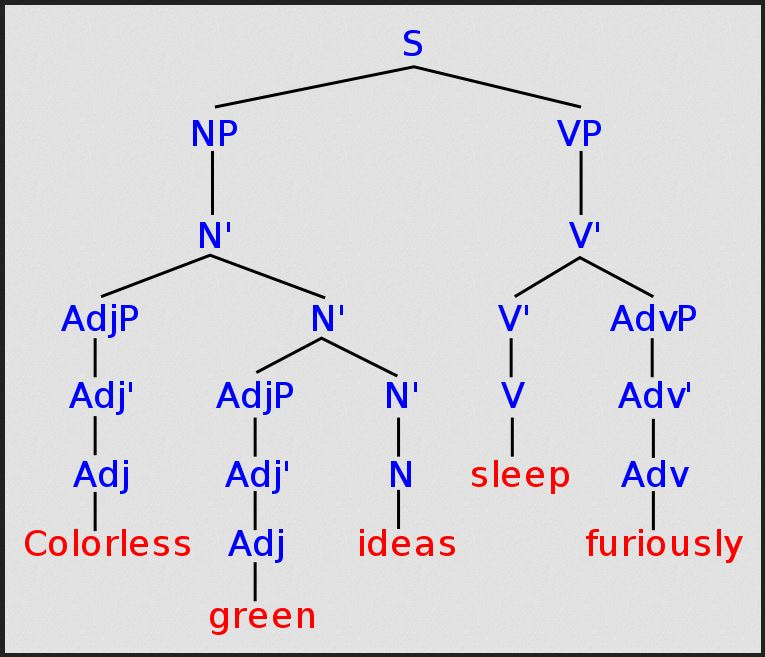
\includegraphics[scale=.3]{material/01colorless}
\end{figure}

\end{frame}


%%%%%%%%%%%%%%%%%%%%%%%%%%%%%%%%%%
\begin{frame}
\frametitle{Was ist Syntax?}

\begin{itemize}
	\item Syntax = Zusammenstellung (griech. \emph{sýn}: \gq{zusammen}, \emph{tàxis}: \gq{Ordnung})
	\item[]
	\item Zusammenstellung und Struktur von Phrasen (und Sätzen) aus kleineren Elementen (Wörtern).
	\item[]
	\item Dabei ist zu beachten:
	\begin{itemize}
		\item dass Phrasen und Sätze \textbf{aus kleineren Teilen} zusammengesetzt sind (Konstituenten),
		\item[]
		\item dass diese Teile unterschiedlicher \textbf{Art} sein können (Kategorie / Wortart),
		\item[]
		\item dass diese Teile \textbf{regelhaft} zusammengesetzt werden,
		\item[]
		\item dass diese Teile an der Stelle, wo sie stehen, eine bestimmte \textbf{Rolle} spielen (Subjekt / Objekt).
 		
	\end{itemize}
	
\end{itemize}

\end{frame}


%%%%%%%%%%%%%%%%%%%%%%%%%%%%%%%%%%
\begin{frame}
\frametitle{Was ist Syntax?}

\begin{itemize}
\item Dabei ist zu beachten, 

\begin{itemize}
	\item \dots dass Phrasen und Sätze aus \textbf{Konstituenten} zusammengesetzt sind,

	\ea
	\gll {Ich schlafe.} = Ich + schlafe\\
	Satz = X + X \\
	\z

\pause

	\item \dots dass diese Teile unterschiedlicher \textbf{Kategorien} sein können,

	\ea 
	\gll {Ich schlafe.} = Ich + schlafe\\
	S = N + V \\
	\z

\end{itemize}

\end{itemize}

\end{frame}


%%%%%%%%%%%%%%%%%%%%%%%%%%%%%%%%%%
\begin{frame}
\frametitle{Was ist Syntax?}

\begin{itemize}
\item Dabei ist zu beachten, 

\begin{itemize}

	\item \dots dass diese Teile \textbf{regelhaft} zusammengesetzt werden,

	\eal 
	\ex[]{Ich schlafe.}
	\ex[*]{Schlafe ich.}
	\zl

\pause

	\item \dots dass diese Teile an der Stelle, wo sie stehen, eine bestimmte \textbf{Rolle} spielen.
			
	\ea
	\gll Ich schlafe.\\
	Subjekt Prädikat\\
	\z
	
\end{itemize}

\end{itemize}

\end{frame}


%%%%%%%%%%%%%%%%%%%%%%%%%%%%%%%%%%
\begin{frame}
\frametitle{Was ist Syntax?}

\begin{itemize}
	\item Eine Minigrammatik:

	\eal 
	\ex Ich schlafe. = Ich + schlafe
\pause	
	\ex	S = N + V 
	\zl

\pause
	
	\eal 
	\ex Ich liebe Syntax.
\pause
	\ex S = N + V + N
	\zl

\pause
		
	\eal 
	\ex Ich zeige Peter Chomsky.
\pause
	\ex S = N + V + N + N 
	\zl
	
\pause
	
	\eal 
	\ex Gestern zeigte Mario Peter Chomsky.
\pause
	\ex S = Adv + V + N + N + N 
	\zl

\pause

	\item Aber: 
	\begin{itemize}
		\item Wie ist S zu definieren?
		\item Was sind die kleineren Bestandteile von S?
		\item Welche Bestandteile sind notwendig und welche hinreichend?
		\item Was ist die Regelmäßigkeit in der Bildung von S?
	\end{itemize}	 	

\end{itemize}

\end{frame}

%%%%%%%%%%%%%%%%%%%%%%%%%%%%%%%%%%
%%%%%%%%%%%%%%%%%%%%%%%%%%%%%%%%%%
\subsection{Linearität und Struktur}
%\frame{
%\frametitle{~}
%	\tableofcontents[currentsection]
%}


%%%%%%%%%%%%%%%%%%%%%%%%%%%%%%%%%%
\begin{frame}
\frametitle{Linearität und Struktur}

\begin{itemize}
	\item \textbf{Linearität} ($\approx$ Reihenfolge) der Wörter in einem Satz ist wichtig!
	
	\ea []{Der kleine Hund sitzt unter dem Stuhl.}
	\z
	
	\ea [*]{Sitzt dem Hund unter Stuhl kleine der.}
	\z

\pause

	\item ABER: \textbf{Struktur} $\neq$ Linearität
	
	\eal 
	\ex Paul sah [den Mann mit dem Fernglas].\\ 
	\vs 
	\ex Paul sah [den 	Mann] [mit dem 	Fernglas].
	\zl
	
	\eal 
	\ex [Alte Frauen] und Männer\\
	\vs
	\ex Alte [Frauen und Männer]
	\zl

	\item Die \textbf{Ambiguität} (Mehrdeutigkeit) der Phrasen liegt in den verschiedenen Möglichkeiten begründet, wie die Wörter sich zu größeren Einheiten kombinieren lassen.

\end{itemize}

\end{frame}


%%%%%%%%%%%%%%%%%%%%%%%%%%%%%%%%%%
\begin{frame}
\frametitle{Linearität und Struktur}

\begin{itemize}
	\item Auch andere Regel können nicht nur mit Bezug auf die Linearität formuliert werden:
	
	\ea Klaus kommt morgen. \hfill (Aussagesatz)
	\z

	\ea Kommt Klaus morgen? \hfill (Entscheidungsfrage)
	\z
	
	\item \textbf{Entscheidungsfragen} (Ja-Nein-Fragen) können scheinbar gebildet werden, indem das zweite Wort im Satz nach vorne verschoben wird.\\
	Aber:

\pause
	
	\ea[]{Der Vater von Klaus kommt morgen.}
	\z
	
	\ea[*]{Vater der von Klaus kommt morgen?}
	\z
	
\end{itemize}

\end{frame}


%%%%%%%%%%%%%%%%%%%%%%%%%%%%%%%%%%
\begin{frame}
\frametitle{Linearität und Struktur}

\begin{itemize}

	\item Entscheidend:
		\begin{itemize}
			\item Manche Elemente gehören enger zusammen als andere: 

			\ea {[Der Vater von Klaus] [kommt] [morgen].}
			\z
			
			\item Rolle der \textbf{Kategorie} von Konstituenten:\\
			\ras Das \textbf{finite} (gebeugte) \textbf{Verb} im Satz muss nach vorne bewegt werden.
			
			\ea {[Kommt]$_i$ der Vater von Klaus t$_i$ morgen?}
			\z
			
		\end{itemize}

\end{itemize}

\end{frame}


%%%%%%%%%%%%%%%%%%%%%%%%%%%%%%%%%%
\begin{frame}
\frametitle{Linearität und Struktur}

\begin{itemize}

	\item Weitere Beispiele (\textbf{Konstituentenfragen}):

	\eal
	\ex Peter liebt \alert{Maria}.
	\ex \alert{Wen$_i$} liebt Peter t$_i$?
	\zl

\pause

	\eal 
	\ex Peter behauptet, dass Maria \alert{Klaus} liebt. 
	\ex \alert{Wen$_i$} behauptet Peter, dass Maria t$_i$ liebt? 
	\zl

\pause

	\eal
	\ex []{Maria kennt den Schriftsteller, der \alert{Die Korrekturen} geschrieben	hat.} 
	\ex [*]{\alert{Was$_i$} kennt Maria den Schriftsteller, der t$_i$ geschrieben hat?} 
	\zl

\pause

	\eal 
	\ex Maria behauptet, dass Klaus gesagt hat, dass er gehört hat, 	dass Irene \alert{Die Korrekturen} gelesen hat. 
	\ex \alert{Was$_i$} behauptet Maria, dass Klaus gesagt hat, dass er gehört hat, dass Irene t$_i$ gelesen hat?
	\zl

\end{itemize}

\end{frame}


%%%%%%%%%%%%%%%%%%%%%%%%%%%%%%%%%%
%%%%%%%%%%%%%%%%%%%%%%%%%%%%%%%%%%
\subsection{Syntax definieren}
%\frame{
%\frametitle{~}
%	\tableofcontents[currentsection]
%}


%%%%%%%%%%%%%%%%%%%%%%%%%%%%%%%%%%
\begin{frame}
\frametitle{Syntax definieren}

\begin{itemize}
	\item Syntax als Disziplin
	\item Syntax als Regelsystem
	\item Syntax als Theorie (oder als Framework)
	\begin{itemize}
		\item Traditionelle Syntax (\ras UE Dt. Grammatik)
		\item Generative Syntax (\ras GK Linguistik)
	\end{itemize}
\end{itemize}

Siehe den Eintrag \gqq{Syntax} in \citep{Glueck05a}

\end{frame}


%%%%%%%%%%%%%%%%%%%%%%%%%%%%%%%%%%
\begin{frame}
\frametitle{Syntax definieren}

\begin{block}{Syntax (Disziplin)}
Syntax ist eine Teildisziplin der Sprachwissenschaft, die sich mit dem Aufbau und den grammatischen Eigenschaften von Phrasen (und Sätzen) auseinandersetzt.
\end{block}

\begin{block}{Syntax (Regelsystem)}
Die \textbf{Syntax einer Sprache} ist das System von Regeln, das alle syntaktisch wohlgeformten Phrasen einer Sprache ableitet und die nicht wohlgeformten Sätze ausschließt.
\end{block}

\end{frame}


%%%%%%%%%%%%%%%%%%%%%%%%%%%%%%%%%%
\begin{frame}
\frametitle{Syntax definieren}

\begin{figure}
\centering
	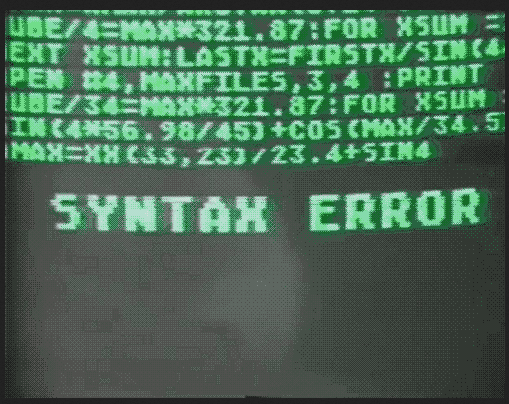
\includegraphics[scale=.7]{material/02syntaxerror}
\end{figure}

\end{frame}


%%%%%%%%%%%%%%%%%%%%%%%%%%%%%%%%%%
\begin{frame}
\frametitle{Syntax definieren}

\begin{block}{Syntax (Regelsystem)}
Die \textbf{Syntax einer Sprache} ist das System von Regeln, das alle syntaktisch wohlgeformten Phrasen einer Sprache ableitet und die nicht wohlgeformten Sätze ausschließt.
\end{block}

	\ea []{Ich schlafe.\label{ex:gramm} \hfill (Wohlgeformt)}
	\z
	
	\ea [*]{Schläfst ich. \label{ex:ungramm} \hfill (Nicht-wohlgeformt)}
	\z
	
\begin{itemize}
	\item Syntaktische Fragen:\\
	\begin{itemize}
		\item Kann ich eine syntaktische Regel ableiten, die \ref{ex:gramm} generiert und \ref{ex:ungramm} ausschließt?
		\item Wie stark kann meine Generalisierung sein?\\
		\ras Mit Bezug auf diesen einen Satz? Auf einen Satztypen? Auf Sätze einer Sprache? Universell?
	\end{itemize}

\end{itemize}

\end{frame}


%%%%%%%%%%%%%%%%%%%%%%%%%%%%%%%%%%
%%%%%%%%%%%%%%%%%%%%%%%%%%%%%%%%%%
\section{Grammatikalität vs. Akzeptabilität}
%\frame{
%\frametitle{~}
%	\tableofcontents[currentsection]
%}


%%%%%%%%%%%%%%%%%%%%%%%%%%%%%%%%%%
\begin{frame}
\frametitle{Grammatikalität}

\begin{itemize}
	\item Was bedeutet \gqq{(nicht-)wohlgeformt}
	
	\ea Schlafe ich
	\z
	
	\ea Sitzt dem Hund unter Stuhl kleine der
	\z
	
	\ea Was behauptet Maria, dass Klaus gesagt hat, dass er gehört hat, dass Irene gelesen hat?
	\z
	
	\ea Ich bin gestern gegangen ins Kino.
	\z
	
	\ea Ich bin glücklich, weil die Studenten lieben Syntax!
	\z
	
	\ea Ins Kino ich gehe heute.
	\z
	
	\ea Gestern ich war im Kino.
	\z
	
	\ea Festschrift oder nicht Festschrift, meinen Geburtstag feiere ich auf jeden Fall. 
	\z
	
\nocite{Finkbeiner&Meibauer14a}
	
\end{itemize}

\end{frame}


%%%%%%%%%%%%%%%%%%%%%%%%%%%%%%%%%%
\begin{frame}
\frametitle{Grammatikalität vs. Akzeptabilität}

\begin{itemize}
	\item \textbf{Ungrammatische} (syntaktisch nicht wohlgeformte) Sätze (Notation:~*) sind zu unterscheiden von Sätzen, die zwar grammatisch, aber
	
	\begin{itemize}
		\item \dots \textbf{inkorrekt verwendet} (Notation: \#) sind:

		\ea A: Hier ist überhaupt nichts langweilig!\\
		B: \# Selbst langweilig ist diese Vorlesung nicht.
		\z
\pause

		\ea A: Diese Vorlesung ist langweilig.\\
		B: Selbst langweilig ist diese Vorlesung nicht!
		\z
		
	\end{itemize}

\end{itemize}
\nocite{Coseriu88a, Fries15a, Repp&Co15a}
\end{frame}


%%%%%%%%%%%%%%%%%%%%%%%%%%%%%%%%%%
\begin{frame}
\frametitle{Grammatikalität vs. Akzeptabilität}

\begin{itemize}
	\item \textbf{Ungrammatische} (syntaktisch nicht wohlgeformte) Sätze (Notation:~*) sind zu unterscheiden von Sätzen, die zwar grammatisch, aber
	
	\begin{itemize}
		
		\item \dots aus \textbf{Verarbeitungsgründen} inakzeptabel (\#) sind:
		
		\ea \# Die, die die, die die, die die Brücken, die für den Verkehr unentbehrlich sind, bauen, unterstützen, belästigen, 		werden bestraft.
		\z
\pause
		
		\ea 
		\ex Die werden bestraft.
		\ex Die, die die belästigen, werden bestraft.
		\ex Die, die die, die die unterstützen, belästigen, werden bestraft.
		\ex Die, die die, die die, die die Brücken bauen, unterstützen, belästigen, werden bestraft.
		\ex Die, die die, die die, die die Brücken, die für den Verkehr unentbehrlich sind, bauen, unterstützen, belästigen, werden bestraft.
		\z

	\end{itemize}

\end{itemize}
\nocite{Coseriu88a, Fries15a, Repp&Co15a}
\end{frame}


%%%%%%%%%%%%%%%%%%%%%%%%%%%%%%%%%%
\begin{frame}
\frametitle{Grammatikalität vs. Akzeptabilität}

\begin{itemize}
	\item \textbf{Ungrammatische} (syntaktisch nicht wohlgeformte) Sätze (Notation:~*) sind zu unterscheiden von Sätzen, die zwar grammatisch, aber
	
	\begin{itemize}
		
		\item \dots aus \textbf{semantischen Gründen} inakzeptabel (\#) sind:
		\ea \# Der Stuhl streichelt den Hund.\\
		(\obj{streicheln} verlangt ein belebtes Subjekt)
		\z
		
		\ea \# Farblose grüne Ideen schlafen wütend. \citep{Chomsky57a}
		\z
		
	\end{itemize}

\end{itemize}
\nocite{Coseriu88a, Fries15a, Repp&Co15a}
\end{frame}


%%%%%%%%%%%%%%%%%%%%%%%%%%%%%%%%%%
\begin{frame}
\frametitle{Grammatikalität \vs Akzeptabilität}

\begin{block}{Akzeptabilität}
Die Akzeptabilität einer Äußerung meint ihre \textbf{beurteilbare Annehmbarkeit} durch einen kundigen Sprecher in der \textbf{Performanz} (Sprachverwendung). Sie ist \textbf{graduierbar} und von verschiedenen Performanzfaktoren abhängig, wie \zB Gedächtnis, Bildungsstand, Alter, Normativität, \dots 
\end{block}

\begin{block}{Grammatikalität}
Die Grammatikalität einer Struktur in einer Sprache meint ihre (Nicht-)\textbf{Generierbarkeit} durch den \textbf{Regelapparat} eines Sprach-Modells (einer Grammatik). Die (Un-)Grammatikalität sprachlicher Strukturen wird dementsprechend ist \textbf{theoriegebunden} und \idR \textbf{binär}. 
Die Grammatikalität bildet die \textbf{Kompetenz} des idealen Sprecher-Hörers ab.
\end{block}

\end{frame}


%%%%%%%%%%%%%%%%%%%%%%%%%%%%%%%%%%
\begin{frame}
\frametitle{Grammatikalität vs. Akzeptabilität}

\begin{itemize}

	\item Grammatikalitätsurteile \ras \textbf{binär}
		
	\ea[*]{Sitzt dem Hund unter Stuhl kleine der.}
	\z
	
	\ea[]{Der kleine Hund sitzt unter dem Stuhl.}
	\z
	
	\item[]
	
	\item Akzeptabilität benötigt für Grammatik(be)schreibung.

	\item Grammatik benötigt für Grammatikalitätsurteile. 

\end{itemize}

\end{frame}


%%%%%%%%%%%%%%%%%%%%%%%%%%%%%%%%%%
%%%%%%%%%%%%%%%%%%%%%%%%%%%%%%%%%%
\section{Deskriptiv \vs Präskriptiv}
%\frame{
%\frametitle{~}
%	\tableofcontents[currentsection]
%}


%%%%%%%%%%%%%%%%%%%%%%%%%%%%%%%%%%
\begin{frame}
\frametitle{Deskriptiv \vs Präskriptiv}

\begin{figure}
\centering
	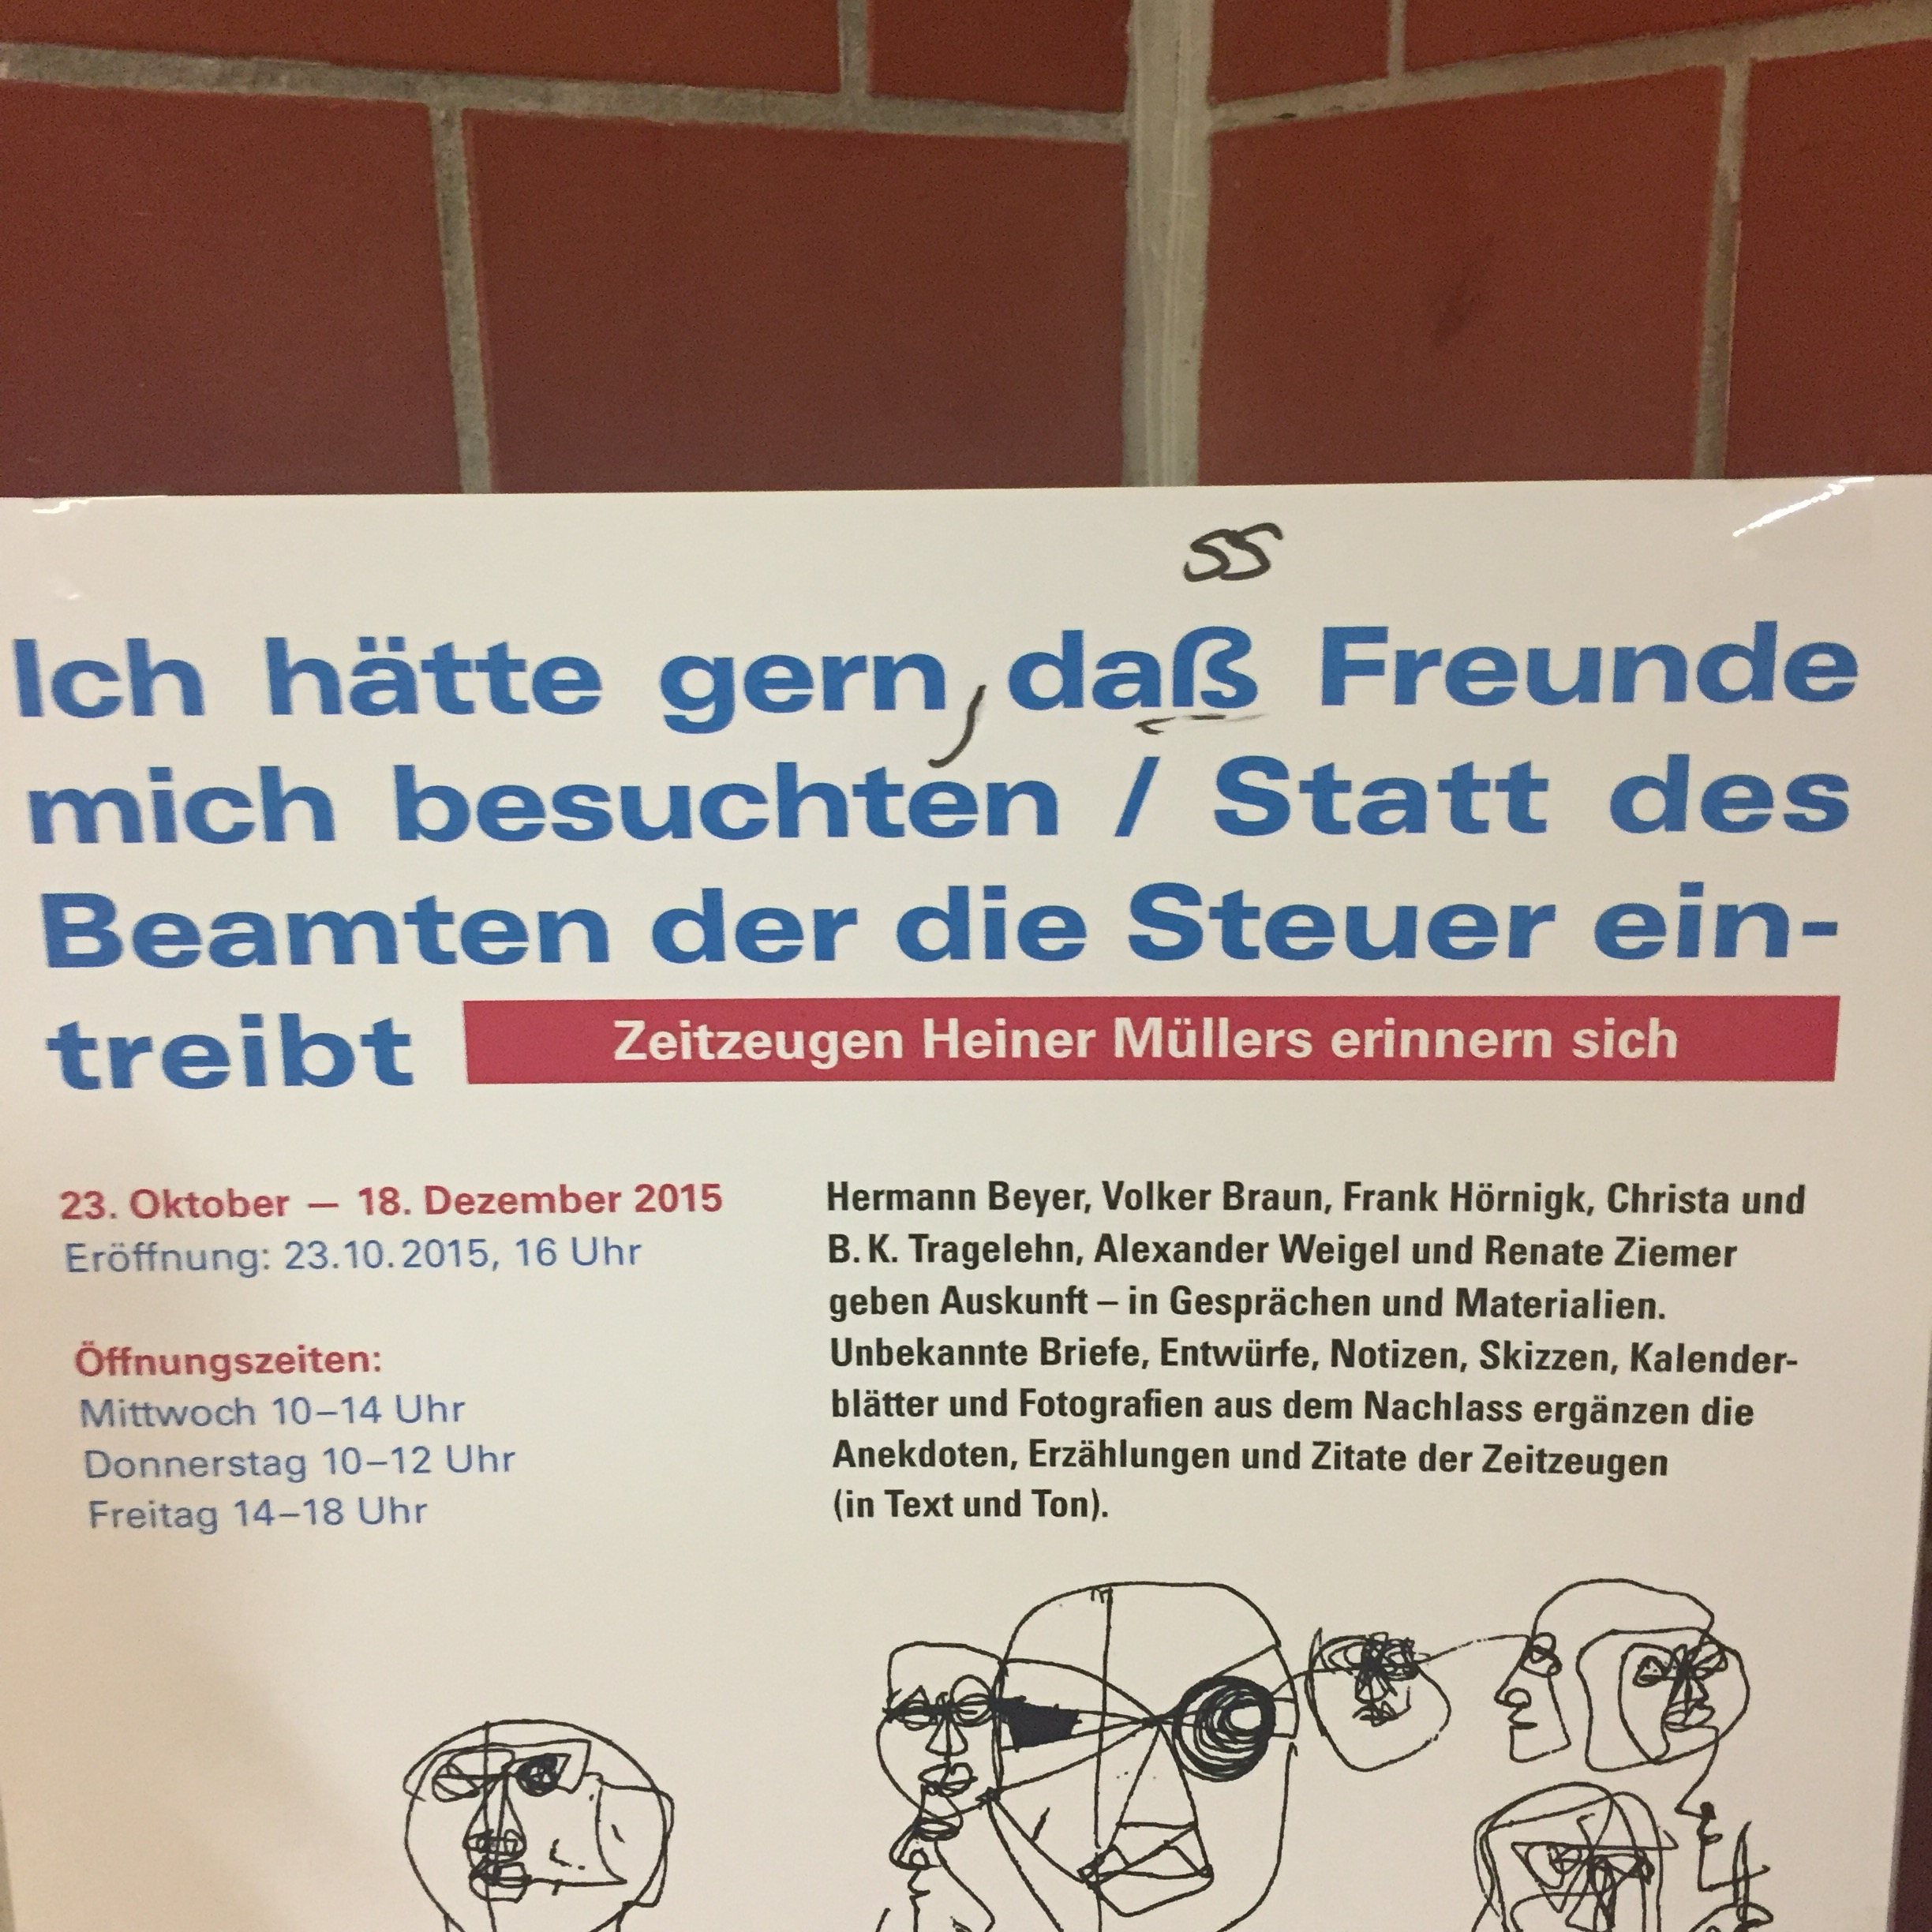
\includegraphics[scale=.07]{material/05praeskriptiv}
	\caption{Das ist präskriptiv.}
\end{figure}

\end{frame}

%%%%%%%%%%%%%%%%%%%%%%%%%%%%%%%%%%
\begin{frame}
\frametitle{Deskriptiv \vs Präskriptiv}

\begin{itemize}
	\item Arbeitsweise in der Linguistik \ras \textbf{Deskriptiv} (beschreibend)
	\begin{itemize}
		\item Ein Phänomen, das kompetente Sprecher produzieren, wird \textbf{beobachtet und beschrieben}. 	
	\end{itemize}
	
	\ea Gestern, ich war im Kino und plötzlich hat es angefangen zu regnen.
	\z
	
	\ea Die theoretische Entwicklung und die praktische Programmierung solcher Betriebssysteme hat sich zu einem neuen Arbeitsgebiet innerhalb der Datenverarbeitung entwickelt. \citep{Goschler14a}
	\z
	
	\item[]
	\item Vorgehensweise von (einigen) Schulgrammatiken und Sprachakademien \ras \textbf{Präskriptiv}
	\begin{itemize}
		\item Es wird \textbf{vorgeschrieben}, wie die Strukturen der Sprache gebildet werden \gqq{müssen}.
	\end{itemize}	
		
	\ea Es heißt nicht \obj{wegen dem Job}, sondern \obj{wegen des Jobs}.	
	\z
	
\end{itemize}

\end{frame}


%%%%%%%%%%%%%%%%%%%%%%%%%%%%%%%%%%
\begin{frame}
\frametitle{Deskriptiv \vs Präskriptiv}

\begin{itemize}
	\item Arbeitsweise in der Linguistik \ras \textbf{Deskriptiv} (beschreibend)
	\begin{itemize}
		\item Ein Phänomen, das kompetente Sprecher produzieren, wird \textbf{beobachtet und beschrieben}. 	
	\end{itemize}
	
	\ea \alert{Gestern, ich} war im Kino und plötzlich hat es angefangen zu regnen.
	\z
	
	\ea Die theoretische Entwicklung und die praktische Programmierung solcher Betriebssysteme \alert{hat} sich zu einem neuen Arbeitsgebiet innerhalb der Datenverarbeitung entwickelt. \citep{Goschler14a}
	\z
		
	\item[]
	\item Vorgehensweise von (einigen) Schulgrammatiken und Sprachakademien \ras \textbf{Präskriptiv}
	\begin{itemize}
		\item Es wird \textbf{vorgeschrieben}, wie die Strukturen der Sprache gebildet werden \gqq{müssen}.
	\end{itemize}		
	
	\ea Es heißt nicht \obj{wegen dem Job}, sondern \obj{wegen des Jobs}.	
	\z
	
\end{itemize}

\end{frame}


%%%%%%%%%%%%%%%%%%%%%%%%%%%%%%%%%%
\begin{frame}
\frametitle{Deskriptiv \vs Präskriptiv}

\begin{itemize}
	\item Präskriptive Regeln \\
	\ras Stilistik (\gqq{schöner} oder \gqq{weniger schön})\\
	oder\\
	\ras Regeln für \gqq{gutes Deutsch}
	\item[]
	\item Linguistik \ras auf der Basis von deskriptiven Beobachtungen
	\item[]
	\item Kompetente Sprecher verwenden ständig Formulierungen wie \obj{wegen dem Job}, aber nie solche wie:

	\ea[*]{Ich bin \alert{wegen der Job} gekommen.}
	\z
	
	\ea[*]{Ich bin \alert{dem wegen Job} gekommen.}
	\z
	
	\ea[*]{Ich bin \alert{wegen Job dem} gekommen.}
	\z
	
\end{itemize}

\end{frame}


%%%%%%%%%%%%%%%%%%%%%%%%%%%%%%%%%%
\begin{frame}
\frametitle{Deskriptiv \vs Präskriptiv}

\begin{itemize}
	\item Kompetente Sprecher verwenden ständig Formulierungen wie \obj{wegen dem Job}, aber nie solche wie:

	\ea[*]{Ich bin \alert{wegen der Job} gekommen.}
	\z
	
	\ea[*]{Ich bin \alert{dem wegen Job} gekommen.}
	\z
	
	\ea[*]{Ich bin \alert{wegen Job dem} gekommen.}
	\z
	
	\item[]
	
	\item Diese Formulierungen sind \textbf{ungrammatisch}, denn sie verletzen Regeln des deutschen grammatischen Systems:
	\begin{itemize}
		\item Präpositionen stehen \emph{vor} Nominalphrasen
		\item Artikel stehen \emph{vor} dem Nominalkomplex
	\end{itemize}	 
\end{itemize}

\end{frame}

